%
% einleitung.tex -- Beispiel-File für die Einleitung
%
% (c) 2020 Prof Dr Andreas Müller, Hochschule Rapperswil
%
% !TEX root = ../../buch.tex
% !TEX encoding = UTF-8
%
\subsection{Kugel\label{geodaeten:section:Linienelement:Kugel}}
\rhead{Linienelemente Beispiele}

In ähnlicher Weise wie im Beispiel mit dem Zylinder lässt sich eine Kugel lokal wie eine flache Ebene darstellen.
Was auf den ersten Blick für sogenannte ``Flat-Earther" ein schwieriges Konzept zu sein scheint, ist intuitiv verständlich:
Zoomt man nahe genug an die Erdoberfläche heran, verschwinden die Krümmungen, und Abstände lassen sich nahezu wie in einem euklidischen Raum berechnen.

In Kugelkoordinaten beschreibt $r$ den Abstand eines Punktes vom Zentrum der Kugel (Radius), $\theta$ den Winkel zur $z$-Achse (Polarwinkel), und $\phi$ den Winkel in der $x$-$y$-Ebene (Azimutwinkel).
Diese Parameter definieren die Position eines Punktes auf der Kugeloberfläche eindeutig, wie in der Abbildung [\ref{geodaeten:figure:Linienelemente:Kugelkoordinaten:Kugelkoordinaten}] dargestellt.

Da wir uns auf der Oberfläche der Kugel befinden, bleibt $r$ konstant, und wir betrachten nur die Winkel $\theta$ und $\phi$.
Wenn ein Punkt nun um einen infinitesimalen Abstand auf der Kugeloberfläche verschoben wird, entstehen Verschiebungen entlang der zugehörigen Basisvektoren:
\begin{equation}
	r \, d\theta
\end{equation}
für die Breitenrichtung und
\begin{equation}
	r \sin\theta \, d\phi
\end{equation} 
für die Längsrichtung.

Weil lokal gerechnet werden kann wie in einem euklidischen Raum, ergibt sich der Abstand zwischen zwei Punkten auf der Kugeloberfläche durch die Anwendung des Pythagoras auf diese jeweiligen infinetsimalen Verschiebungen.

Das Linienelement $ds$ für die Oberfläche der Kugel kann daher als
\begin{equation}
	ds^2 = r^2 \, d\theta^2 + r^2 \, \sin^2\theta \, d\phi^2
\end{equation}
beschrieben werden.

\begin{figure}
	\centering
	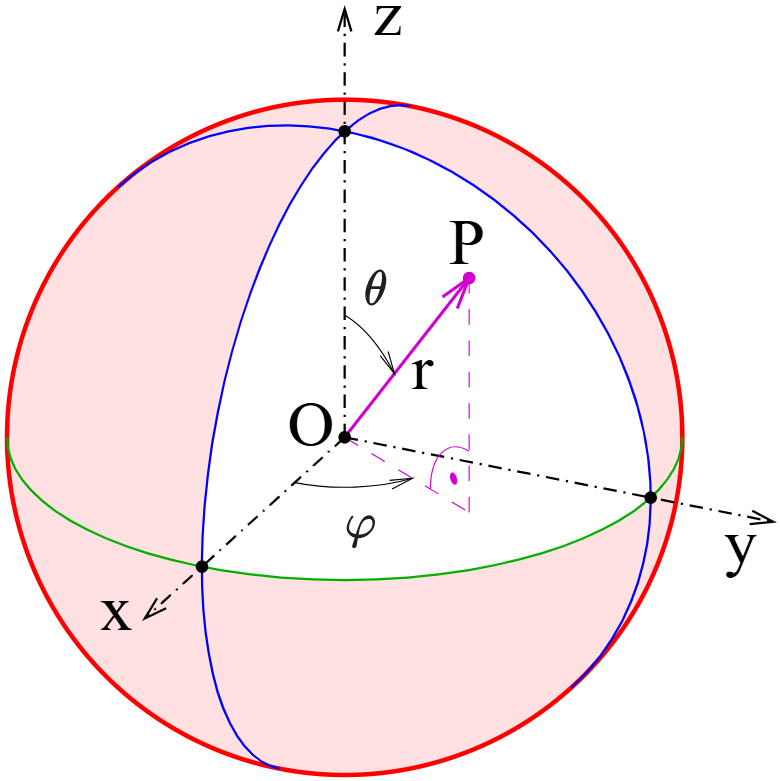
\includegraphics[width=6cm]{papers/geodaeten/Abbildungen/Linienelemente/LinKugel1}
	\caption{Kugelkoordinaten mit Radius $r$, Polarwinkel $\theta$ und Azimutwinkel $\phi$}
	\label{geodaeten:figure:Linienelemente:Kugelkoordinaten:Kugelkoordinaten}
	\cite{geodaeten:Kugelkoordinaten}
\end{figure}
